\chapter{Performance Analysis}\label{cap:rendimiento}
\noindent In this chapter qosh performance will be evaluated deployed on a real cluster. The execution environment will be described first and the metrics collected will be analyzed and put in context thereafter.

\section{Testing Environment}\label{sec:entornodeprueba}
\noindent Figure \ref{fig:clusterdespliegue} shows how the cluster is configured. The leftmost part of the figure shows the Cloud Controller; the rightmost, the Cloud Node. The Cloud Controller has been installed the full OpenStack Folsom package --- except for Cinder, Swift and Quantum as they will not used ---, plus MySQL, Fabric and Qpid as message broker. In the Cloud Node only the bare minimum to support VM execution has been installed --- OpenStack Compute and KVM. Other functional requirements of the Cloud Node, like access control or VM image download, are delegated to the Cloud Controller via Qpid.

\begin{figure}[tbp]
\begin{center}
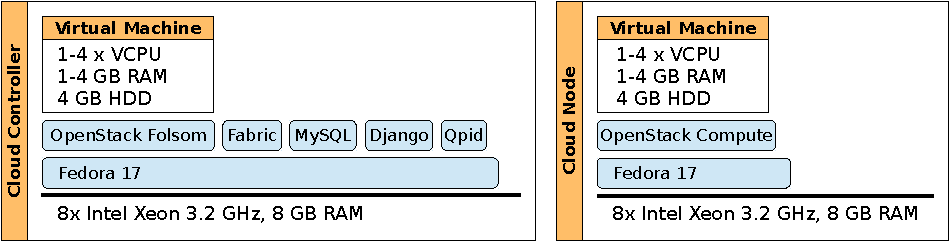
\includegraphics[width=0.99\textwidth]{imagenes/038.pdf}
 \caption{Deployment morphology}
\label{fig:clusterdespliegue}
\end{center}
\end{figure}

Regarding the physical layer, both nodes posses the same hardware configuration: Octa core Intel Xeon processor @ 3.2 GHz with VT-x, 8 GB of RAM, 200 GB SATA 3 Gb/s 7200 RPM and Gigabit networking interface.

The Hadoop virtual image, whose creation procedure is described in section \ref{subsec:maquinavirtual}, will be used in the VMs to execute MapReduce workflows. Figure \ref{fig:clusterdespliegue} shows the Hadoop VM in context. This instance will be  provided with 1 to 4 GB of RAM and the same number of VCPUs to assess qosh's scaling. The deployment has been configured to allow Hadoop to address all the memory in the VM --- except for those addresses in use by the OS and the JVM.

\section{Testing Methodology}\label{sec:metodologiaprueba}
\noindent This section contains both in and out scalability analysis and a study on qosh behavior on increasing input sizes. To evaluate how qosh scales, a MapReduce workflow large enough to stress every instance in the virtual cluster, will be fed to Hadoop; the workflow will count the words in 62.5 MB of plain text.

To actually assess horizontal scalability, the size of the virtual cluster will progressively be doubled starting from one instance up to four. To test vertical scalability, two VMs will be initially spawned with 1 GB of RAM each, to have their RAM and VCPU count doubled on each test case until reaching 4 GB of RAM and 4 VCPUs. Finally, to evaluate the running time tendency, the input text size will be doubled from the original 62.5 MB to 250 MB.

As Glance and Compute cooperate to cache images, the time required to start an instance will be longer the first time it launches, effectively skewing results. To get rid of those divergences, the instances on each flavor will be \emph{warmed} by starting and destroying them once before taking measures.

\emph{A priori}, the expected variance of the timings between executions is small enough to consider \emph{ten} to be a representative number of runs for each test case --- this hypothesis will be validated \emph{a posteriori} on analyzing the results. To measure timings, the code will include a set of time marks that will help take apart the following times:

\begin{description}
    \item[Deploying:] Time elapsed since the virtual cluster creation request is send until every instance is accessible.
    \item[Configuring:] Time required to establish the Hadoop execution environment. It comprises the time to configure the virtual Hadoop cluster plus the time to distribute input data onto HDFS.
    \item[MapReducing:] Time dedicated by Hadoop to execute the \emph{wordcount} workflow.
    \item[Cleaning:] Time required to wipe out the execution environment. It does not include the time it takes OpenStack to completely remove the instances.
    \item[Total:] Time required by the whole process to complete. It is not the result of adding the previous four times.
\end{description}

It should be noted that the timings shown are the averaged results of the ten executions in each case.

\section{Analyzing the Results}\label{sec:analisisresultados}

\begin{figure}[tbp]
\begin{center}
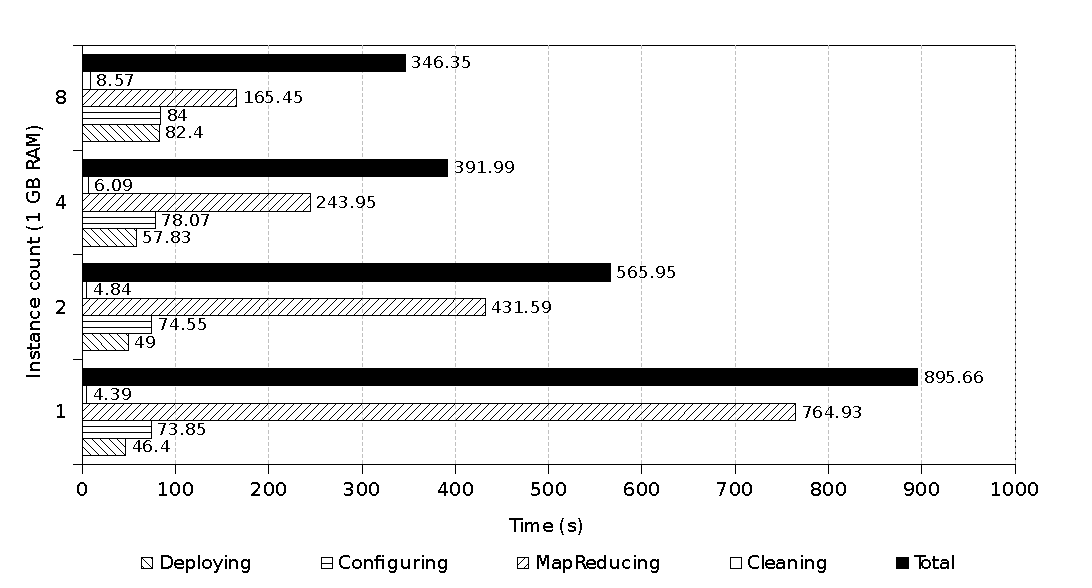
\includegraphics[width=0.98\textwidth]{imagenes/039bw.pdf}
\caption{Scaling out}
\label{fig:eschorizontal}
\end{center}
\end{figure}

\noindent Figure \ref{fig:eschorizontal} shows the evolution of the different timings as the instance count increases from one to eight. It may be observed that deployment, configuring and cleaning time increase with the number of instances deployed, meanwhile processing time is reduced. I.e, the time required for a virtual cluster to deploy, configure and delete every instance depends \emph{only} on its size. On the other hand, MapReducing time --- and thus total time --- is also bound to input size. Figure \ref{fig:escvertical} presents the tendency of the five timings as the cluster is scaled in from 1 GB of VCPU and RAM to 4 each.

\begin{figure}[tbp]
\begin{center}
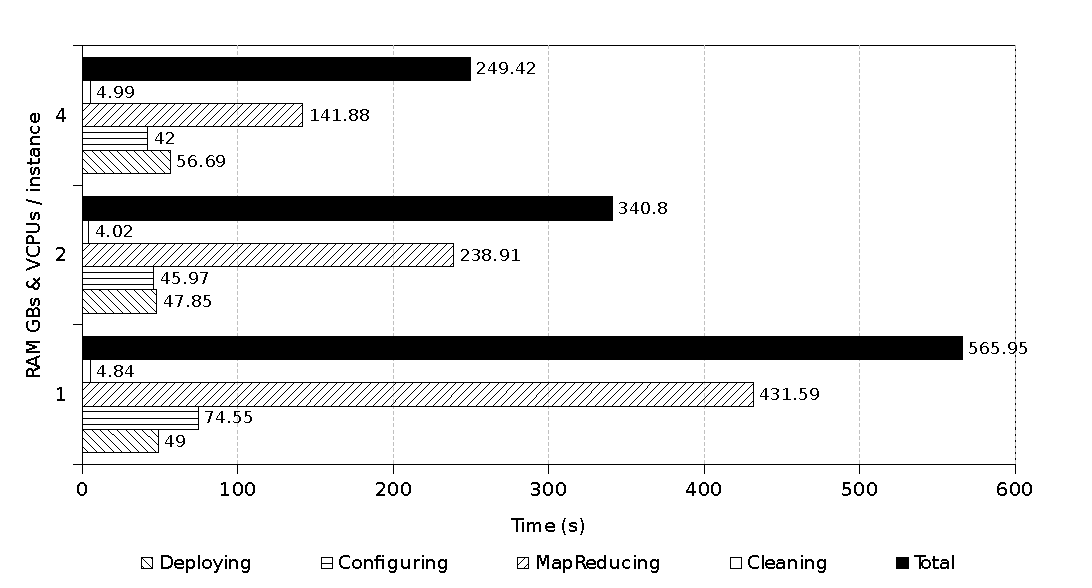
\includegraphics[width=0.98\textwidth]{imagenes/041bw.pdf}
\caption{Scaling in}
\label{fig:escvertical}
\end{center}
\end{figure}

It should be highlighted from figure \ref{fig:escvertical} that deploying and cleaning times are approximately flat even though the instances are made larger. I.e., the difficulty to deploy or delete a virtual cluster in our environment depends exclusively on the number of instances or virtual nodes --- conclusion we had drawn earlier. Configuring times in this case are reduced, for the instances are more capable computationally --- while testing horizontal scaling revealed that configuring time increased proportionally with the cluster size.

In light of the results, it can be concluded that qosh behaves more efficiently on vertical scaling versus horizontal scaling. This fact is specially evident when contrasting the extreme testing cases from figures \ref{fig:eschorizontal} and \ref{fig:escvertical}: eight instances, 1 GB of RAM and 1 VCPU each and 4 GB of RAM and 4 VCPUs respectively. Both test cases deploy a virtual cluster with 8 VCPUs and 8 GB of RAM over the physical infrastructure. Yet, total execution time is almost \emph{28\%} smaller with two larger instances.

\begin{figure}[tbp]
\begin{center}
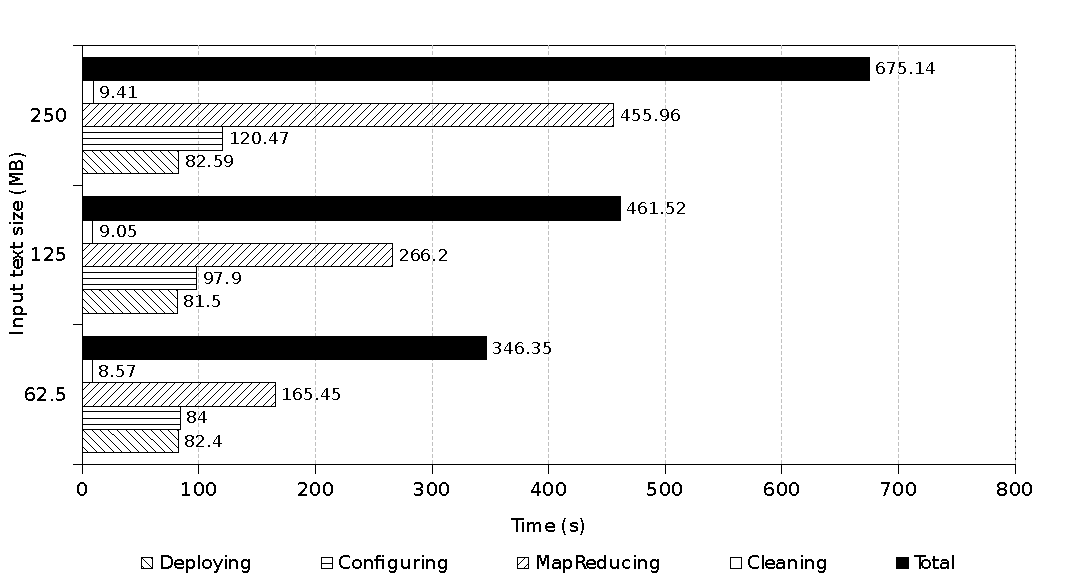
\includegraphics[width=0.98\textwidth]{imagenes/042bw.pdf}
\caption{Input size versus execution time}
\label{fig:evotemporal}
\end{center}
\end{figure}

Figure \ref{fig:evotemporal} shows the tendency on execution times when increasing the input size. As expected, MapReducing and total times increase with input size but in a smaller proportion. Deploying and cleaning times stay almost constant on each case, while configuring time increases slightly as it covers decompressing and distributing the input files over the cluster.
